%% objective

I combined the Synexpression Territories (STs) approach with genome-wide coding-region polymorphism data (from the DGRP database) and the coding-region divergence between \textit{D. yakuba} and \textit{D. melanogaster} in order to estimate the  proportion of adaptive non-synonymous substitutions ($\omega_{\alpha}$) in the genes expressed in each ST (n=589 genes; III, Methods).
	\nomenclature{$\omega_{\alpha}$}{Proportion of adaptive non-synonymous substitutions}

Using this approach, I could chart a spatial map of natural selection acting on \textit{Drosophila}'s embryo anatomy.
I complemented this with a analysis using available annotation of gene expression (n=2,835 genes) using a controlled vocabulary of anatomical structures from the BDGP database \citep{Tomancak2007}.

%% results %%%%%%%%%%%%%%%%%%%%%%%%%%%%%%%%%%
The results showed a few STs with significant higher or lower $\omega_{\alpha}$ (permutation test; III, Methods)

%% high OmegaA
\subsection{STs or anatomical terms with high $\omega_{\alpha}$}
STs 13 and 32 (ST number comes from the hierarchical clustering algorithm), which showed a higher $\omega_{\alpha}$, seem to correspond to the forming foregut and hindgut (stage 11-12) and to the CNS (stage 13-16) respectively.
To explore if ST 32 high $\omega_{\alpha}$ was indeed related to the CNS, I separated the genes CNS or not-CNS related.
I found that both groups showed a high $\omega_{\alpha}$, which suggests that in addition to the CNS, another structure in the anterior region would be under positive selection.
 Using the anatomical terms approach, no anatomical terms related to the CNS were found to have high $\omega_{\alpha}$ with the initial criteria.
I therefore applied a more stringent criterion to consider genes as part of an anatomical term (before a gene could have a maximum of seven anatomical terms associated instead of a more stringent number of three) and found that `Embryonic brain' showed high $\omega_{\alpha}$ (permutation test, p = 0.046).
Also, with the anatomical terms approach, I found that genes associated with `Gonads', in the last stage, clearly showed evidence of adaptive evolution (III, Figure 2).

The evidence of adaptation in in agreement with previously reported high rates of adaptive substitution in the testes \citep{Akashi1994,Civetta1995,Nuzhdin2004,Proschel2006}

%% low omegaA
\subsection{STs or anatomical terms with low $\omega_{\alpha}$}
STs 20 and 29 with showed low $\omega_{\alpha}$, seem to correspond to the forming midgut (stage 11-12) and to the forming larval digestive system (stage 13-16) respectively.
Similar results are found when using the anatomical term approach, as low $\omega_{\alpha}$ was found in many anatomical terms related to the digestive system in the last stage: `Embryonic midgut', `Embryonic salivary gland', `Embryonic hindgut', `Embryonic proventriculus'. 
Also, combining three related anatomical terms, `Embryonic foregut', `Embryonic epipharynx' and `Embryonic hypopharynx', that separately did not have enough genes to be considered in the analysis, showed low $\omega_{\alpha}$. 

The lack of adaptive change in the forming digestive system might reflect their relative enrichment in metabolic genes \citep{Marianes2013}. The coding regions of metabolic genes have been found to be more conserved than non-metabolic genes \citep{Peregrin-Alvarez2009}.


%%%%%%%%%%%%%%%%%%%%%%%%%%%%%%%%%%%%%%%%%%%%%%%%%%%%%%%%
\begin{figure}[h]
  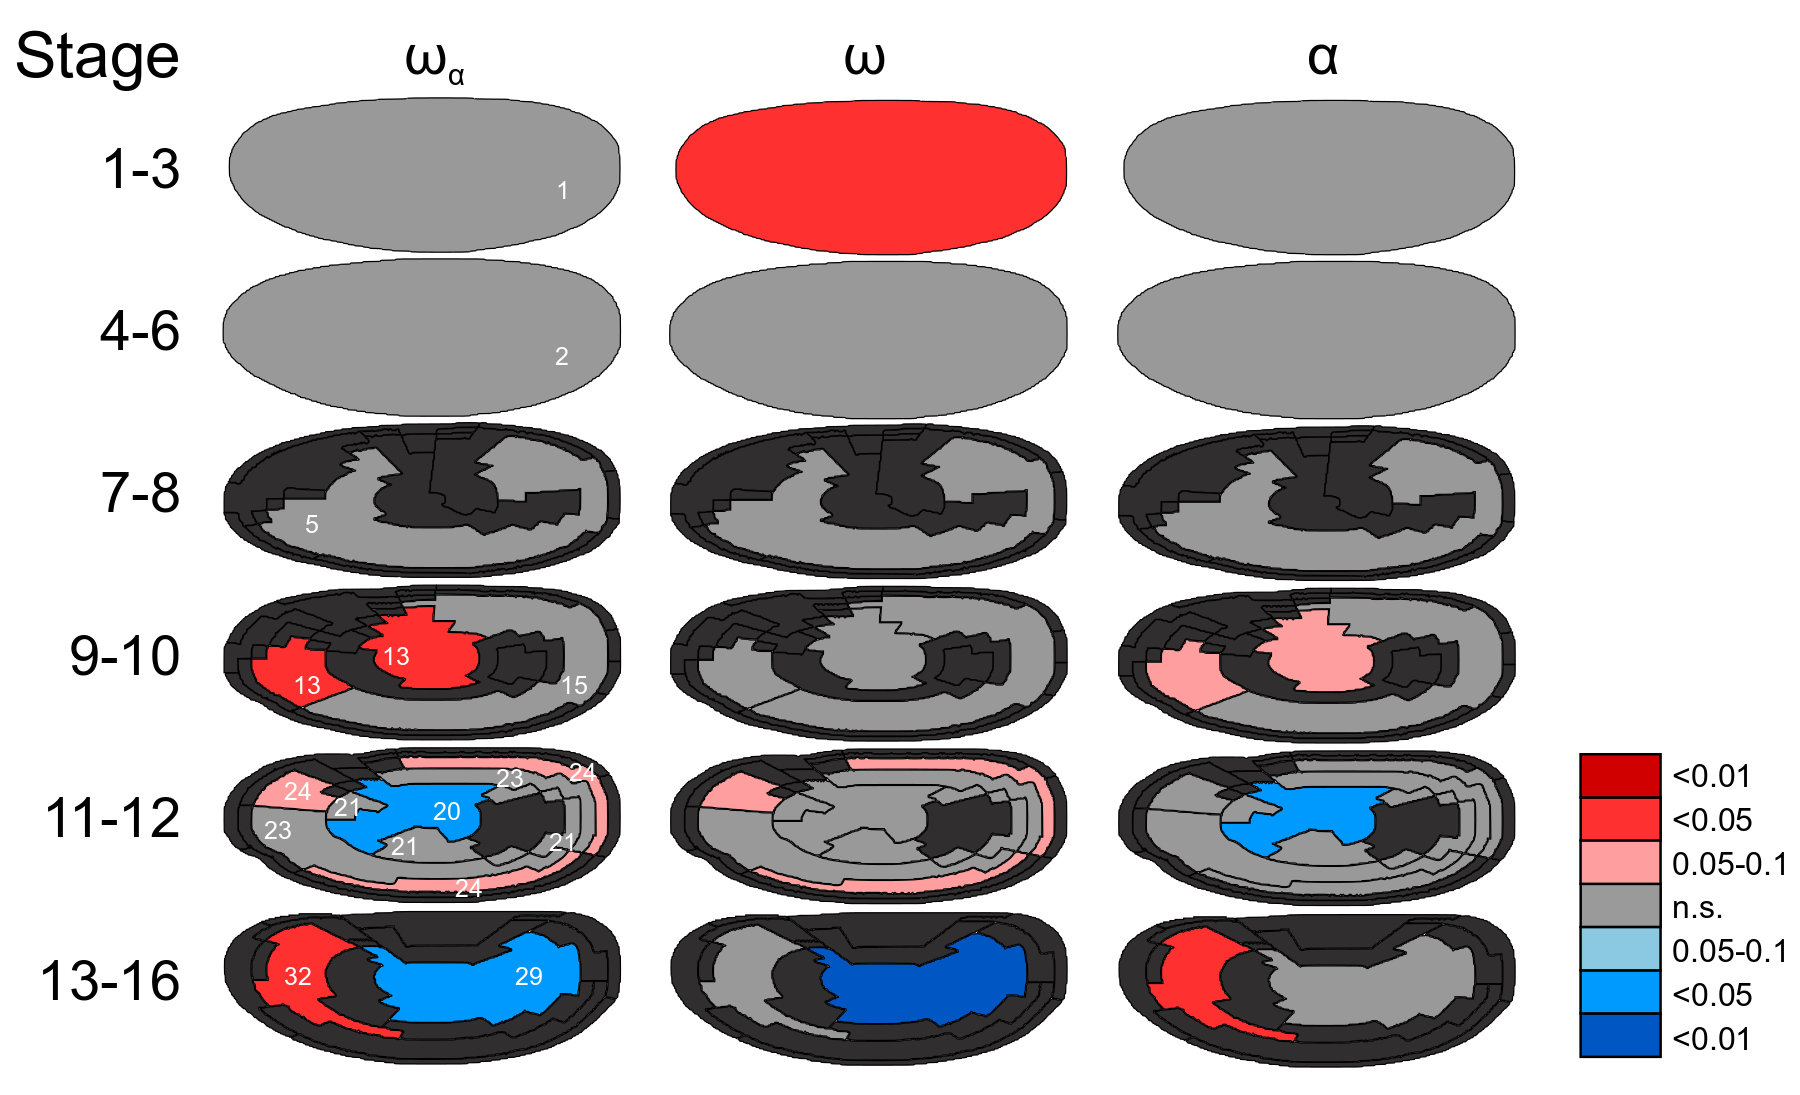
\includegraphics[width=0.8\textwidth]{./Images/Art-III/OmegaA_territories.png}
  \centering
  \caption{\textbf{$\omega_{\alpha}$ on embryonic territories over space and time.}
   Territories drawn in red in the central column mark significantly high $\omega_{\alpha}$ while those in blue mark significantly low $\omega_{\alpha}$ in space in each of the 6 developmental stages (rows). Other columns depict $\alpha$, the proportion of base substitutions fixed by natural selection, and $\omega$, the rate non-synonymous substitutions relative to the mutation rate. 
  Territories in dark gray are territories without enough specific genes to be analyzed. The statistical was calculated by a permutation test using all the genes analyzed (see Material and methods). Territory 13 in stage 9-10 ($\omega_{\alpha}$: 0.059, p = 0.045). Territory 20 from stage 11-12 ($\omega_{\alpha}$: 0.022, p = 0.048; $\alpha$: 0.259, p = 0.028). Territory 24 from stage 11-10 ($\omega_{\alpha}$: 0.070, p = 0.061). Territory 29 from stage 13-16 ($\omega_{\alpha}$: 0.037, p = 0.047; $\omega$: 0.074, p < 0.001). Territory 32 from stage 13-16 ($\omega_{\alpha}$: 0.068, p = 0.044; $\alpha$: 0.71, p = 0.04).
  }
  \label{fig:Art-III-OmegaA_territories}
\end{figure}
%%%%%%%%%%%%%%%%%%%%%%%%%%%%%%%%%%%%%%%%%%%%%%%%%%%%%%%%


\subsection{Transcriptome age index}

We also measured the phylogenetic age \citep{Drost2015} of the genes expressed in each territory, that is, the phylogenetic level at which orthologs for a gene are found (e.g., if a gene has orthologs among eukaryota the phylogenetic age is older than if a gene has orthologs only among Drosophilids). 

The territories where we found low rates of coding-region adaptive evolution express genes that are, on average, older than the genes expressed elsewhere (Figure 3). Similar results are found for anatomical structures (Figure S2).

We also found that in the latest stages the mean phylogenetic age of the genes expressed in the endoderm is lower than that of the genes expressed in other germ-layers, specially compared to the ectoderm (Figure 3). Similar results were found by \citep{Domazet-Loso2007} but without comparing stages.

Our analysis also shows that the embryo regions with high rates of adaptive substitution have low codon bias \citep{Sharp1991,Betancourt2002,Haerty2007} and, as previously reported \citep{Plotkin2011}, regions with high codon bias have high levels of gene expression (measured by RNA as reported in modENCODE \citep{Graveley2011} and averaged per region; see Materials and methods) (see Figure 4).

This latter correlation, however, was larger for regions with low $\omega_{\alpha}$ than for regions with high $\omega_{\alpha}$ (Figure 5A). Figure 5 shows that genes in regions with high $\omega_{\alpha}$ exhibit low codon bias relative to gene expression levels. The same relationship between $\omega_{\alpha}$ and codon bias is found in territory 32, the territory showing the stronger evidence of adaptive substitution (Figure 5).
